\section{基本可行解与最优解}
\label{sec:opt-lp-basic-solutions}

在平面上，顶点是两条边界直线的交点，求它只需解一个二元一次方程组。标准型~\eqref{eq:opt-lp-standard}生活在$\mathbb R^n$中，有$m$个等式；若再让$n-m$个坐标取零，剩下$m$个未知数、$m$个方程，一般也能解出唯一一点。本节把这一观察整理成“基”和“基本可行解”，证明它们恰好是可行域的极点，并证明只要最优值有限，就能在有限个基本可行解中找到最优解。这为单纯形法在基之间组织搜索提供了依据。

\subsection{基、基本解与基本可行解}
\label{sec:opt-lp-bases}

\paragraph{满行秩假设}
用“选$m$列解方程”来描述点之前，先要保证等式系统没有多余的方程。由线性方程的解结构，$\bm A\bm x=\bm b$有解当且仅当$\operatorname{rank}\bm A=\operatorname{rank}[\bm A\ \bm b]$；有解时，若$\operatorname{rank}\bm A=r<m$，可以挑出$r$个线性无关的行，其余各行都是它们的线性组合，删去其余行不改变解集。这里用到的秩判别、消元与LU分解，可参考\BookChapterRef{chap:linear-equations-and-optimization}{卷一“线性方程与矩阵方程”章}。若方程不相容，可行域是空集，问题已经回答。因此在讨论基之前，我们总假设$\bm A\in\mathbb R^{m\times n}$满行秩，即$\operatorname{rank}\bm A=m\le n$。实际计算中并不需要预先做这一步，第~\ref{sec:opt-lp-two-phase}节的第一阶段会在求可行点的同时发现冗余行。

\begin{definition}[基与基本可行解]
\label{def:opt-lp-basic-feasible}
设$\bm A$满行秩。若$m$个指标组成的集合$B\subseteq\{1,\dots,n\}$使对应各列构成的方阵$\bm A_B$可逆，就称$B$为一个基，$\bm A_B$为\term{基矩阵}（basis matrix），其余指标记为$N$。令$\bm x_N=\bm 0$，并由$\bm A_B\bm x_B=\bm b$解出$\bm x_B=\bm A_B^{-1}\bm b$，所得的$\bm x$称为基$B$对应的\term{基本解}（basic solution）；$x_j$（$j\in B$）称为\term{基变量}（basic variable），$x_j$（$j\in N$）称为\term{非基变量}（nonbasic variable）。若还有$\bm x_B\ge\bm 0$，就称$\bm x$为\term{基本可行解}（basic feasible solution）。若某个基变量取零，称这个基本可行解是退化的。
\end{definition}

基本解满足全部等式，但不一定满足非负约束；只有$\bm x_B\ge\bm 0$时它才落在可行域中。

\begin{example}[资源模型的六个基本解]
\label{ex:opt-lp-six-basic-solutions}
在例~\ref{ex:opt-lp-resource-standard}中$m=2$、$n=4$，四列中任取两列都线性无关，共有$\binom42=6$个基。以$B=\{1,4\}$为例，令$x_2=x_3=0$，方程组变为$2x_1=4$、$x_1+x_4=4$，解得$x_1=2$、$x_4=2$，对应平面上的点$(2,0)$，第二种原料还剩$2$个单位。同样算得：$B=\{3,4\}$给出$(0,0)$，$B=\{2,3\}$给出$(0,2)$，$B=\{1,2\}$给出$(4/3,4/3)$，这四个是基本可行解。$B=\{1,3\}$令$x_2=x_4=0$，第二个方程给出$x_1=4$，第一个方程给出$x_3=4-8=-4<0$，基本解$(4,0)$用掉的第一种原料超过库存；$B=\{2,4\}$类似地给出$(0,4)$与$x_4=-4$。图~\ref{fig:opt-lp-basic-solutions}把六个基本解画在平面上：它们正是四条边界直线两两的交点，其中落在四边形上的四个恰好是四个顶点。
\end{example}

\begin{figure}[!htbp]
  \centering
  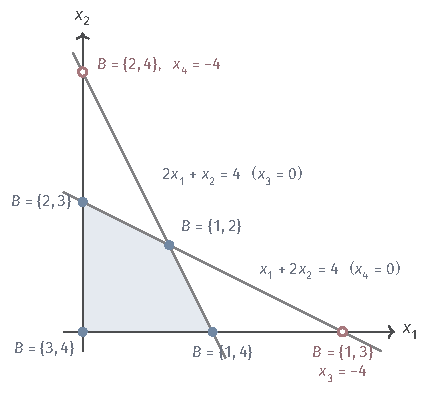
\includegraphics[width=72.796mm]{figures/03-optimization-evolution-and-signals/01-optimization/tikz/c2-basic-solutions/figure.pdf}
  \caption{资源分配例的六个基本解。每个基$B$指定两个取正值的候选变量，其余两个变量取零，即令两条边界同时取等号；$x_3=0$与$x_4=0$分别对应两条灰线，$x_1=0$与$x_2=0$对应两条坐标轴。蓝色实心点是四个基本可行解，即可行域的四个顶点；红色空心点是两个基本解，它们各有一个松弛变量为负，落在可行域外。}
  \label{fig:opt-lp-basic-solutions}
\end{figure}

\paragraph{退化：多个基，同一个点}
基与点不一定一一对应。在资源模型中再加一条市场限制$x_1\le2$，引入松弛变量$x_5$，得到$m=3$、$n=5$的标准型。可行域没有变化，因为$x_1\le2$在原四边形上本来就成立；但顶点$(2,0)$现在有三条边界同时经过：$x_2=0$、$2x_1+x_2=4$与$x_1=2$。这一点对应的$\bm x=(2,0,0,2,0)^\top$只有$x_1$和$x_4$两个正分量，而基要有三个指标。把第三个指标取为$3$、$5$或$2$都能使基矩阵可逆，三个基$\{1,3,4\}$、$\{1,4,5\}$、$\{1,2,4\}$给出同一个点，每个基中都有一个取零的基变量。所以“基变量的个数”$m$与“正分量的个数”不必相同，后者可以更少。第~\ref{sec:opt-lp-degeneracy}节会看到，这种退化会让单纯形法换了基却停在原地。

\paragraph{基本可行解就是极点}
下面的定理把代数对象（基本可行解）与几何对象（极点）连起来，并给出一个不需要先找基的判别：只看正分量所在的列。

\begin{theorem}[基本可行解与极点]
\label{thm:opt-lp-bfs-extreme}
设$\bm A$满行秩，$\bm x\in P$，记$J=\{j:x_j>0\}$。以下三条等价：
\begin{enumerate}
  \item $\bm x$是$P$的极点；
  \item 列$\{\bm a_j:j\in J\}$线性无关；
  \item $\bm x$是某个基对应的基本可行解。
\end{enumerate}
\end{theorem}

\begin{proof}
(1)$\Rightarrow$(2)：若这些列线性相关，存在不全为零的系数$w_j$（$j\in J$）使$\sum_{j\in J}w_j\bm a_j=\bm 0$。把$\bm w$在$J$以外的分量补为零，就有$\bm A\bm w=\bm 0$且$\bm w\ne\bm 0$。由于$x_j>0$对$j\in J$成立，取足够小的$\varepsilon>0$可使$\bm x\pm\varepsilon\bm w\ge\bm 0$，又$\bm A(\bm x\pm\varepsilon\bm w)=\bm b$，所以$\bm x\pm\varepsilon\bm w$都可行，且它们不相等，$\bm x$是二者的中点。这与$\bm x$是极点矛盾。

(2)$\Rightarrow$(3)：线性无关的列至多$m$个，所以$|J|\le m$。$\bm A$满行秩，它的列张成$\mathbb R^m$，可以从其余列中补进若干列，把$\{\bm a_j:j\in J\}$扩充为$\mathbb R^m$的一组基，相应指标集记为$B\supseteq J$。于是$\bm A_B$可逆，$N=\{1,\dots,n\}\setminus B$中的指标都不在$J$中，$\bm x_N=\bm 0$；再由$\bm A\bm x=\bm A_B\bm x_B=\bm b$得$\bm x_B=\bm A_B^{-1}\bm b$。$\bm x$可行，故$\bm x_B\ge\bm 0$，它是基$B$的基本可行解。

(3)$\Rightarrow$(1)：设$\bm x$是基$B$的基本可行解，且$\bm x=\lambda\bm u+(1-\lambda)\bm v$，$\bm u,\bm v\in P$，$\lambda\in(0,1)$。对$j\in N$，$0=x_j=\lambda u_j+(1-\lambda)v_j$，而$u_j,v_j\ge0$，只能$u_j=v_j=0$。于是$\bm A_B\bm u_B=\bm b$，$\bm u_B=\bm A_B^{-1}\bm b=\bm x_B$，即$\bm u=\bm x$；同理$\bm v=\bm x$。所以$\bm x$是极点。
\end{proof}

证明的第一步给出了一个今后反复使用的操作：若可行点的正分量所在列线性相关，就能找到方向$\bm w\ne\bm 0$，满足$\bm A\bm w=\bm 0$且只在正分量上非零，沿$\pm\bm w$都能走一小段而不离开可行域。定理也提醒我们，“手里有一个可行点”与“手里有一个可用的基”是两回事：一般可行点的正分量可能多于$m$个，它不是基本可行解，要从它得到一个基还需要计算。

\subsection{最优基本可行解与最优面}
\label{sec:opt-lp-optimal-bfs}

图~\ref{fig:opt-lp-resource-polygon}中最优解落在顶点上。下面证明这在标准型中总成立：只要可行域非空、目标有下界，就存在作为基本可行解的最优解。证明不预先假设最优解存在，而是把任意可行点“推”到一个不更差的基本可行解上。

\begin{lemma}[推向基本可行解]
\label{lem:opt-lp-push-to-bfs}
设$\bm A$满行秩，$P\ne\varnothing$，且$\bm c^\top\bm x$在$P$上有下界。则对每个$\bm x\in P$，存在基本可行解$\widehat{\bm x}$，使$\bm c^\top\widehat{\bm x}\le\bm c^\top\bm x$。
\end{lemma}

\begin{proof}
对正分量个数$|J|$（$J=\{j:x_j>0\}$）作归纳。若列$\{\bm a_j:j\in J\}$线性无关，由定理~\ref{thm:opt-lp-bfs-extreme}，$\bm x$本身是基本可行解。否则，像定理证明中那样取$\bm w\ne\bm 0$，满足$\bm A\bm w=\bm 0$且$w_j=0$对$j\notin J$成立。必要时把$\bm w$换成$-\bm w$，可使$\bm c^\top\bm w\le0$。

先排除一种情形：$\bm c^\top\bm w<0$且$\bm w\ge\bm 0$。此时对一切$t\ge0$，$\bm x+t\bm w\ge\bm 0$且$\bm A(\bm x+t\bm w)=\bm b$，目标值$\bm c^\top\bm x+t\bm c^\top\bm w$随$t$趋于$-\infty$，与有下界矛盾。若$\bm c^\top\bm w=0$且$\bm w\ge\bm 0$，则把$\bm w$换成$-\bm w$，仍有$\bm c^\top\bm w=0\le0$，而且$-\bm w$有负分量。因此总可以假设$\bm c^\top\bm w\le0$，并且$\bm w$至少有一个负分量。

令
\[
  t^\star=\min\Bigl\{\frac{x_j}{-w_j}:w_j<0\Bigr\}>0,\qquad
  \bm x'=\bm x+t^\star\bm w.
\]
$t^\star$的取法保证$\bm x'\ge\bm 0$，又$\bm A\bm x'=\bm b$，所以$\bm x'\in P$，且$\bm c^\top\bm x'=\bm c^\top\bm x+t^\star\bm c^\top\bm w\le\bm c^\top\bm x$。$\bm w$只在$J$上非零，$J$以外的分量保持为零，而取到最小值的那个分量变为零，所以$\bm x'$的正分量个数严格减少。由归纳假设，$\bm x'$可以推到一个基本可行解$\widehat{\bm x}$，$\bm c^\top\widehat{\bm x}\le\bm c^\top\bm x'\le\bm c^\top\bm x$。
\end{proof}

\begin{theorem}[最优基本可行解的存在性]
\label{thm:opt-lp-optimal-bfs}
设$\bm A$满行秩。若标准型~\eqref{eq:opt-lp-standard}可行且目标在$P$上有下界，则最优值能够取到，并且至少有一个最优解是基本可行解。特别地，非空的$P$至少有一个极点。
\end{theorem}

\begin{proof}
基至多有$\binom nm$个，所以基本可行解只有有限个；对$P$中任一点应用引理~\ref{lem:opt-lp-push-to-bfs}，知它们至少有一个。在有限个基本可行解中取目标值最小的$\bm x^\star$。对任意$\bm x\in P$，引理给出基本可行解$\widehat{\bm x}$，使$\bm c^\top\bm x\ge\bm c^\top\widehat{\bm x}\ge\bm c^\top\bm x^\star$。所以$\bm x^\star$是全局最优解。最后一句取$\bm c=\bm 0$即得。
\end{proof}

这个定理是线性规划区别于一般优化问题的地方：一般问题中“有下界”推不出“下确界能取到”，例如$e^{x}$在$\mathbb R$上有下界$0$却取不到；在标准型线性规划中，有限的最优值总能取到。证明用到了两点：$\bm x\ge\bm 0$使可行域不含直线，引理中总有一个分量会先降到零；线性目标沿直线的变化是线性的，要么能朝不变差的方向推进，要么出现无下界的射线。

\paragraph{枚举基的代价}
定理说明，原则上可以列出全部基，解出基本解，丢掉不可行的，再比较目标值。资源模型只有$6$个基，这样做毫无困难。但基的个数$\binom nm$随规模急剧增长：$n=100$、$m=50$时约为$1.0\times10^{29}$。即使每秒检查$10^{12}$个基，也远远无法完成。我们需要只在“相邻”的基之间移动、并且每一步都让目标不变差的方法，这就是下一节的单纯形法。

\paragraph{最优解未必都是基本可行解}
定理只断言存在一个最优的基本可行解，并不是说每个最优解都是基本可行解。图~\ref{fig:opt-lp-optimal-face}比较了同一可行域上的两个目标。最大化$3x_1+2x_2$时，最优解只有顶点$(4/3,4/3)$。改为最大化$2x_1+x_2$时，目标等值线与边$2x_1+x_2=4$平行，最优值为$4$，两个顶点$(2,0)$与$(4/3,4/3)$都最优，它们的连线上每一点也都最优。例如二者的中点$(5/3,2/3)$对应标准型中的$\bm x=(5/3,2/3,0,1)^\top$，有三个正分量，多于$m=2$，所以它不是基本可行解，却同样最优。这里的最优面是两个最优顶点的全部凸组合，即一整条边。因此，若求解方法只报告一个顶点，它回答了“最优值是多少”和“一个最优解是什么”，并没有回答“最优解是否唯一”。

\begin{figure}[!htbp]
  \centering
  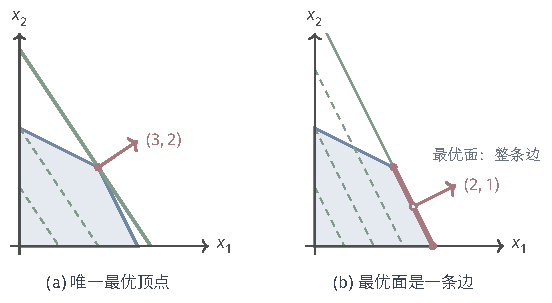
\includegraphics[width=93.419mm]{figures/03-optimization-evolution-and-signals/01-optimization/tikz/c2-optimal-face/figure.pdf}
  \caption{同一可行域上的唯一最优解与多个最优解。(a) 最大化$3x_1+2x_2$，绿色实线为最优等值线$3x_1+2x_2=20/3$，它只接触顶点$(4/3,4/3)$。(b) 最大化$2x_1+x_2$，绿色虚线为等值线$2x_1+x_2=1,2,3$，最优等值线$2x_1+x_2=4$与一条边重合；红色粗线上的点都最优，空心点$(5/3,2/3)$是其中一个不是顶点的最优解。}
  \label{fig:opt-lp-optimal-face}
\end{figure}
